\chapter{Evaluation}

\section{Discussion}
Within the discussion the results of the different \ac{SHS} components and the overall system will be treated, postulating with supporting evidence what may have lead to certain outcomes. Different future avenues are outlined to gain further insight.

\subsection*{Step Detection}
For step detection, the implementation of \cref{algo:step_detect} was compared with that of \citet{Salvi2018}, who had continued the work of \cite{Harle2013}.  \par 
Within the step counting results, there were two observations made. Firstly, the total number of steps counted by both implementations was similar in all carrying modes, many of which had 5\% or less in counting error. There was a large outlier for both cases with the step counting in the back pocket of "user1". Researchers attribute this to the pocket being loose and allowing the phone to rebound when a step was taken \cite{Salvi2018}. This would introduce nefarious components in the accelerometer signal, leading to false positives. \citet{Brajdic2013} encountered similar problems with this carrying position, hypothesizing that the relaxing of the gluteus maximus during locomotion could influence the acceleration trace.\\
The similarity between the two approaches is further underlined by the results in which the time difference between a step detection and its closest ground truth point was calculated. Many detections were within 0.1 seconds from their closest ground truth point. Here the best performing option also changed per carrying mode and person.\par 
Original data was also gathered for step counting and evaluated using the devised method. Here similar results were found to the opensource data. Bad performance in the back pocket was also found, with the best performance being when the smartphone is held in hand. The bad performance in the back pocket further underlines the reliability of step detection in this carrying mode. \par  
The third metric for "unique" step detection was explained and applied, in an attempt to filter out detections detecting the same step. In contrast to the previous metric, this indicated that \cref{algo:step_detect} had more "unique" steps, which are steps closest to a ground truth point, without another detection at the same distance. This would suggest that the current implementation is better at determining the time at which a step occurs. \\
This difference between the two implementations can potentially be explained by the goal and implementation of the \citet{Salvi2018} approach. This research was focused on only \textit{step counting} and did no measurements themselves to determine how close their detections were to the actual steps. Any eventual lag would not affect the step counting performance, as long as the steps are counted. Their android implementation, the output of which was indicated in the validation set, may have had some form of lag. The lag would shift all points, potentially putting them in between step occurrences. This could cause two of them to be in an interval around a ground truth point, which the metric then considers not "unique". \par 

With step detection, the goal was to get similar or better performance than \cite{Salvi2018} . The same parameters found through a variable space search in \cite{Salvi2018}, were used in the step detection method, with the idea that the same performance would be reached. While the results seem to show similar results, it may be worthwhile to run the same variable to check that the parameters are indeed the best for step detection.

\subsection*{Step Length Estimation}
The step length estimation results show that the general linear relationships outlined in \cite{Vezocnik2019} were found, however, the accuracy claimed was not, performing worse than expected. This is most likely caused by the difference in step detection methods, which \cite{Vezocnik2019} does not state explicitly. A similar small scale experiment was performed. Results from this indicate that normal to slow walking worked best with the approach of \cite{Tian2016}, with a tendency to underestimate the distance traveled. \par 

In contrast to the open-source data, the exact number of steps taken for the tunable parameter dataset was known. The number of steps detect was either exactly the same or two steps off. This suggests that the step detection is working correctly and that the methods may be lacking. It may be worthwhile to test the other algorithms outlined by \cite{Vezocnik2019} to see if there are any other differences between the outcomes. 

\newpage


\subsection*{Orientation Estimation}

\begin{itemize}
	\item There is no concrete way with the data available to check how well the EKF estimate is working in comparison to reality. Only comparing to the android system is possible.
	\item trial 3 and trial 6 had the largest yaw difference of the trials. The yaw traces between the android system and EKF can be found in \cref{fig:202011181708yawdifferencebetweenmethods} and \cref{fig:202011181705yawdifferencebetweenmethods}
	\item EKF for trial 6 has a weird jump and slowly gets back to the estimate of the android system. Not clear what is causing this. \textcolor{red}{How should I handle this further?}
	\item for trial 3 there seems to be a slight offset between the orientation estimations.
\end{itemize}

\begin{figure}[H]
	\centering
	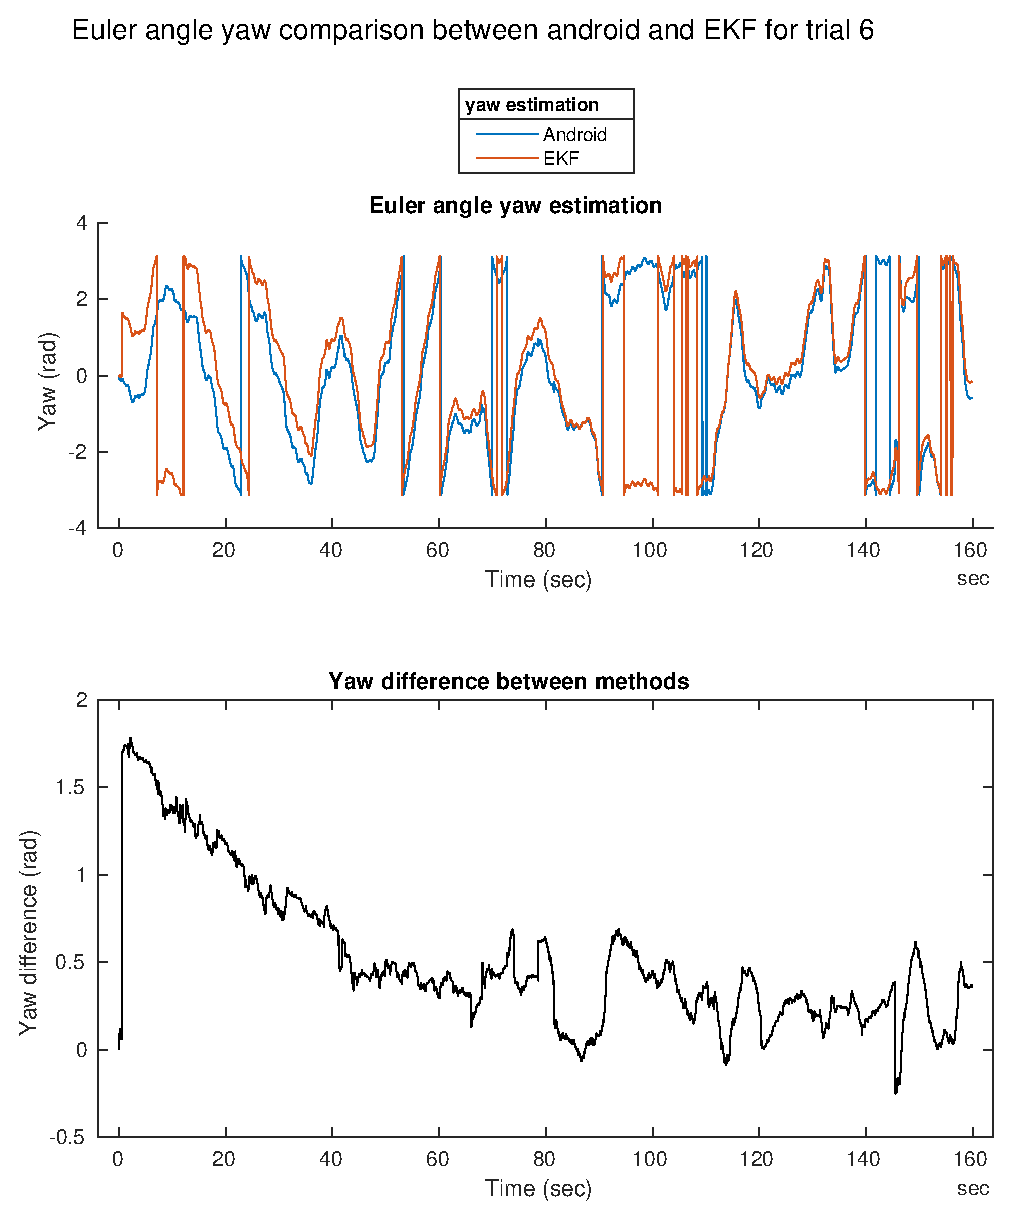
\includegraphics[width=0.7\linewidth]{images/20201118_1708_Yaw_difference_between_methods}
	\caption{}
	\label{fig:202011181708yawdifferencebetweenmethods}
\end{figure}
\begin{figure}[H]
	\centering
	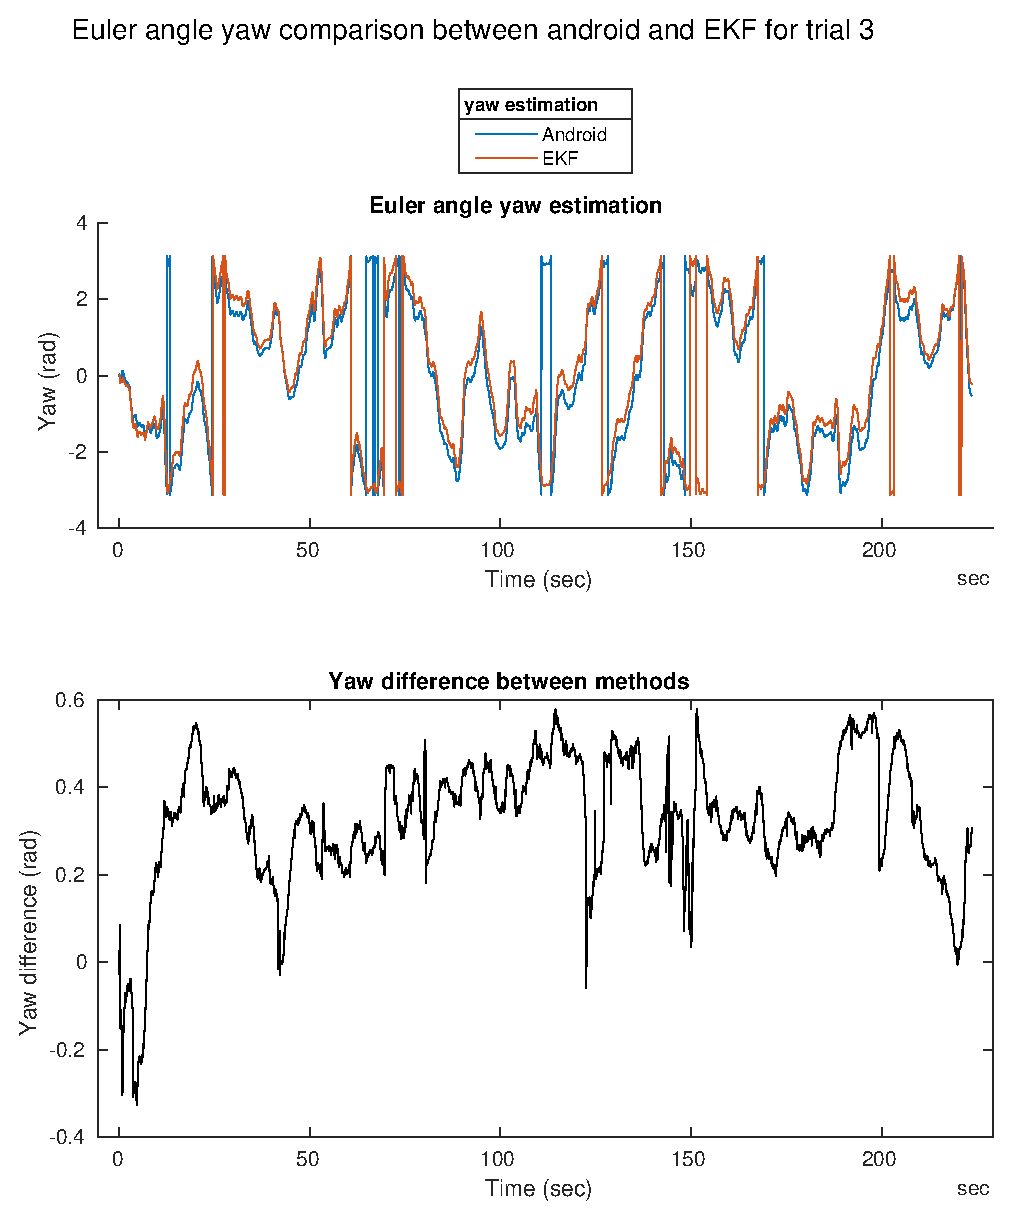
\includegraphics[width=0.7\linewidth]{images/20201118_1705_Yaw_difference_between_methods}
	\caption{}
	\label{fig:202011181705yawdifferencebetweenmethods}
\end{figure}



\newpage
\subsection*{Overall System Performance}

\begin{itemize}
	\item Using door interaction that were manually indicated, 4 out of 6 trials were able to complete all itterations. They do have a difference in median RMSE value and the spread between itterations. The reasoning why this is occurring can be spotted in the trajectories that the particle filter calculate.  
	\item The particle for trial 1 and 2 complete all itterations, it does not follow the complete trajectory. This can be seen in  \cref{fig:shspf_trial1_shs_gt_comparison} where the structure circled in green is circled by the rough estimate but not by the particle filter. For \cref{fig:shspf_trial2_shs_gt_comparison} the particle filter seems to walk too far and is unable to make the correct turn.
	\item trial 3 and 7 are able to follow the whole route. corresponding to lower RMSE values, the outputs are shown in \cref{fig:shspf_trial7_shs_gt_comparison}.
	\item theory that step length estimation is over estimating distance traveled in some cases. This can be cause by turning not having the same displacement as a straight step.
	\item give a table of the distance walked according to rough video estimate and what the shs estimated.
	\item Comparing the results when activity recognition is not used, the use of activity recognition can potentially improve localization, since more trials are able to survive the whole SHS trajectory when it is than when it is not. This is most apparent with trial 7, where with activity recognition it is able to complete the whole root, while with out it only one itteration survives, which is also has a large error with the video estimate. The results also shows that it is not a necessity in some cases to use this form of measurement update, with trial 1 and 2 completing all itterations with similar RMSE values as when AR is used.
	\item When using the AR method outlined in \cref{chap:method}, trial 3 was unable to complete all itterations. The itterations that were completed had a large range of RMSE. This is likely caused by false positives. Plots still need to be made to show this.
\end{itemize}


\begin{figure}[H]
	\centering
	\begin{subfigure}[t]{.45\textwidth}
		\centering
		\begin{tikzpicture}
			\node[anchor=south west,inner sep=0] (image) at (0,0) {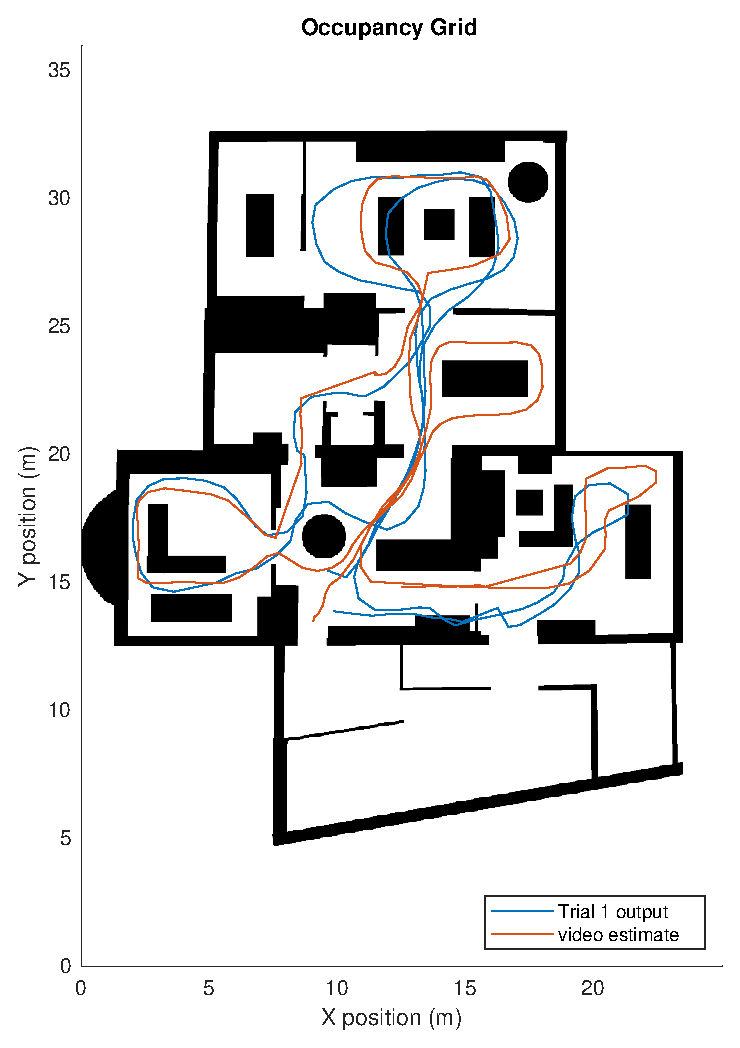
\includegraphics[width=0.9\textwidth]{images/20201118_1900_trial1_output_2}};
			\begin{scope}[x={(image.south east)},y={(image.north west)}]
				\draw[green,ultra thick,rounded corners] (0.6,0.625) rectangle (0.73,0.66);
			\end{scope}
		\end{tikzpicture}		
		\caption{trajectory comparison}
		\label{fig:shspf_trial1_on_map}
	\end{subfigure}
	\begin{subfigure}[t]{.45\textwidth}
		\centering
		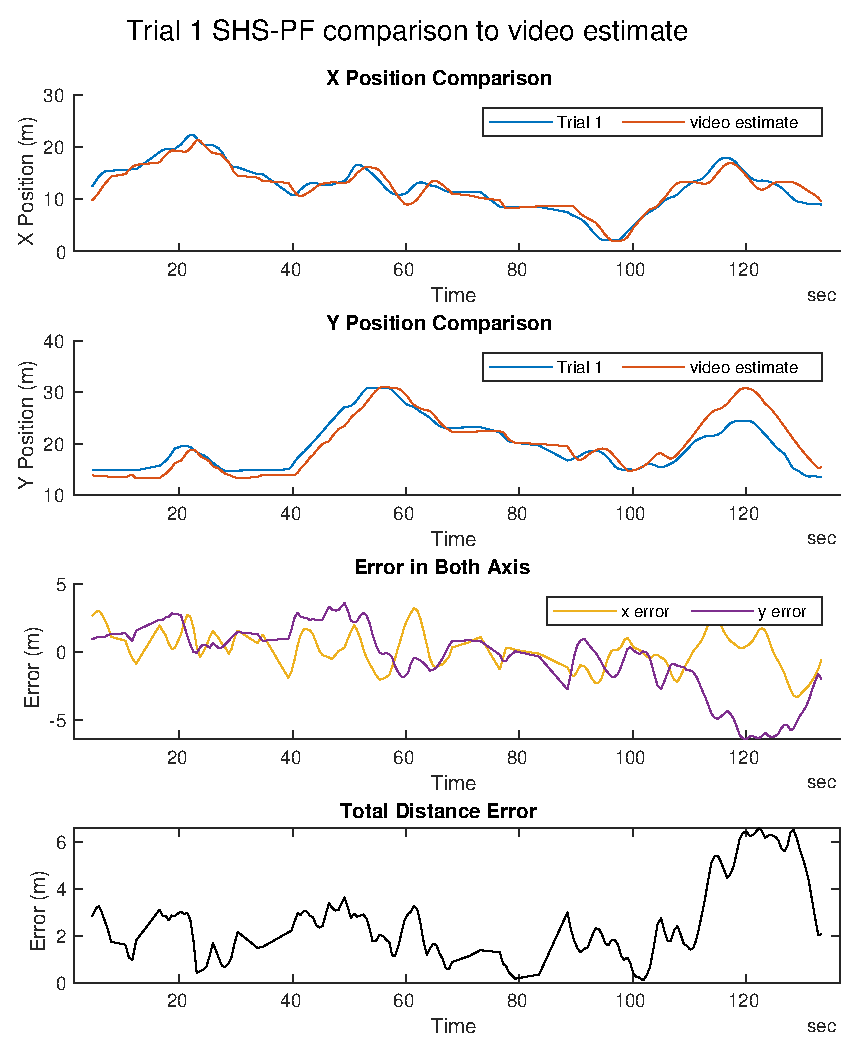
\includegraphics[width=\linewidth]{images/20201118_1900_trial1_output_1}
		\caption{axis comparison}
		\label{fig:shspf_trial1_comparison}
	\end{subfigure}
	\setlength{\belowcaptionskip}{-20pt}
	\caption{SHS-PF comparison of trial 1 with ground truth}
	\label{fig:shspf_trial1_shs_gt_comparison}
\end{figure}
\begin{figure}[H]
	\centering
	\begin{subfigure}[t]{.45\textwidth}
		\centering
		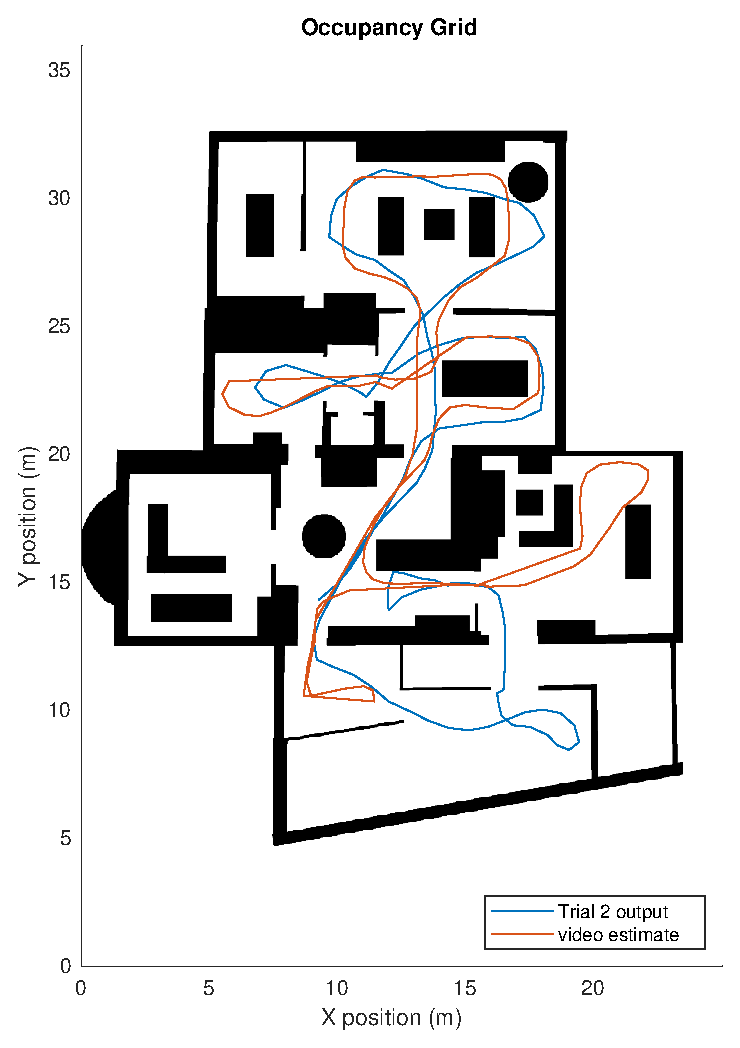
\includegraphics[width=0.9\linewidth]{images/20201118_1902_trial2_output_2}
		\caption{trajectory comparison}
		\label{fig:shspf_trial2_on_map}
	\end{subfigure}
	\begin{subfigure}[t]{.45\textwidth}
		\centering
		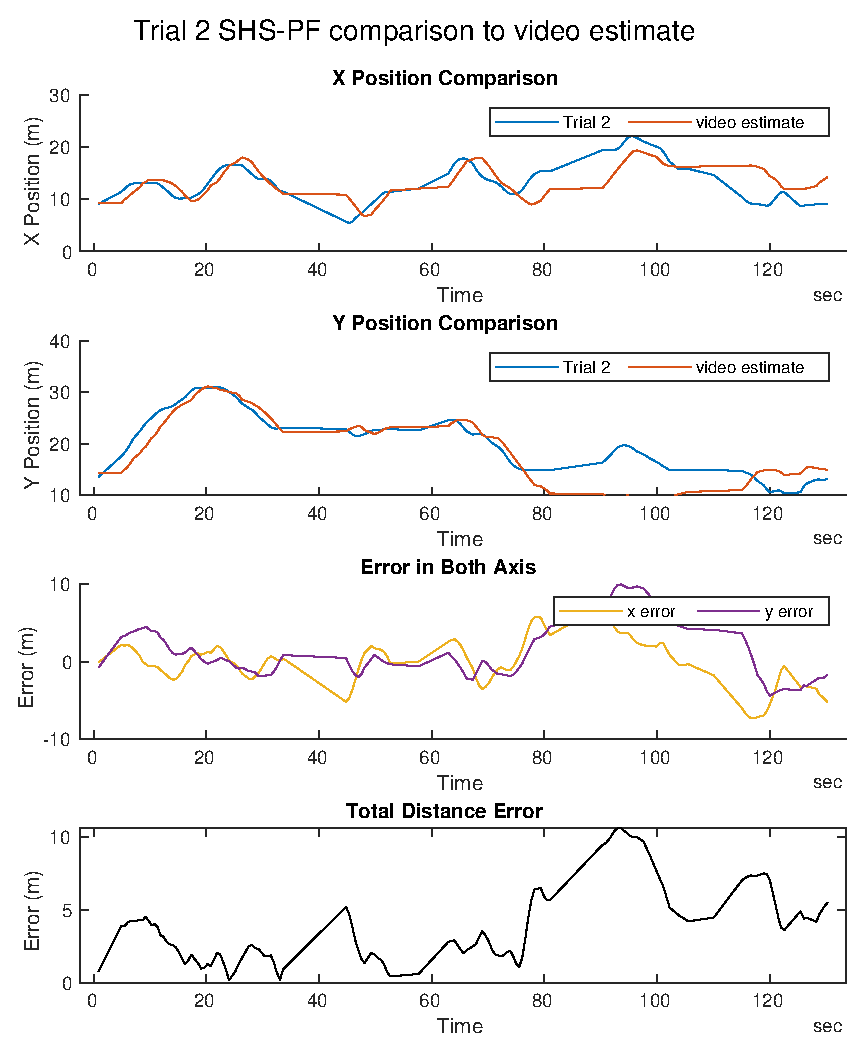
\includegraphics[width=\linewidth]{images/20201118_1902_trial2_output_1}
		\caption{axis comparison}
		\label{fig:shspf_trial2_comparison}
	\end{subfigure}
	\caption{SHS-PF comparison of trial 2 with ground truth}
	\label{fig:shspf_trial2_shs_gt_comparison}
\end{figure}

\begin{figure}[H]
	\centering
	\begin{subfigure}[t]{.45\textwidth}
		\centering
		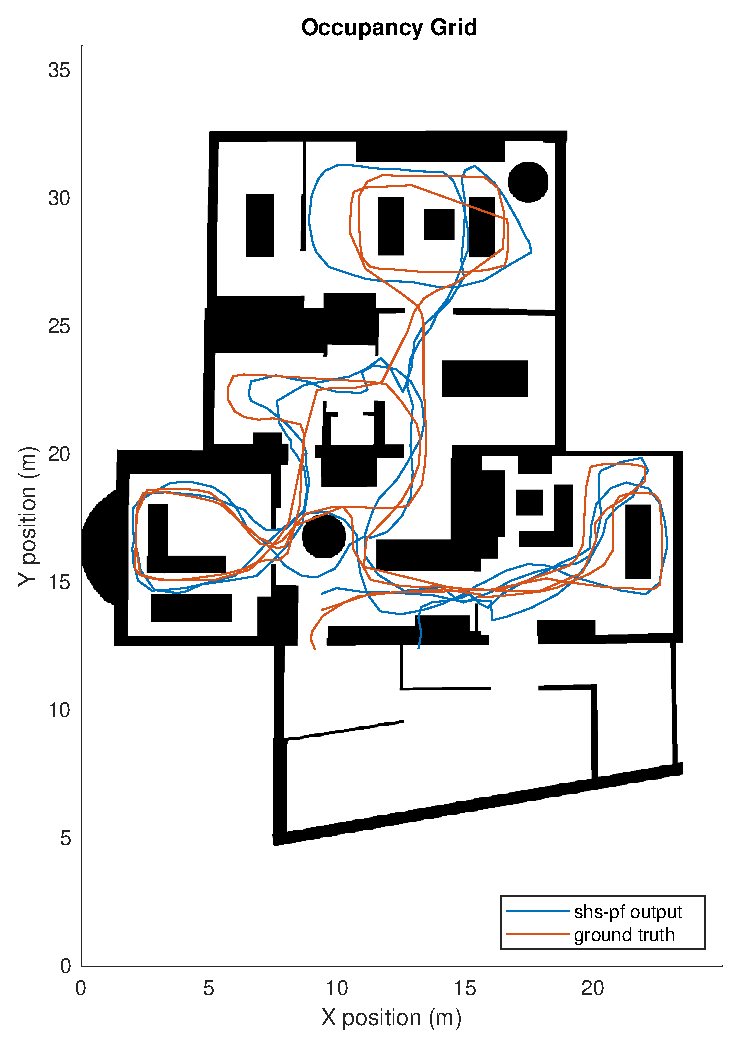
\includegraphics[width=0.9\linewidth]{images/20201029_1804_shs-pf_trial_3_2}
		\caption{trajectory comparison}
		\label{fig:shspf_trial3_on_map}
	\end{subfigure}
	\begin{subfigure}[t]{.45\textwidth}
		\centering
		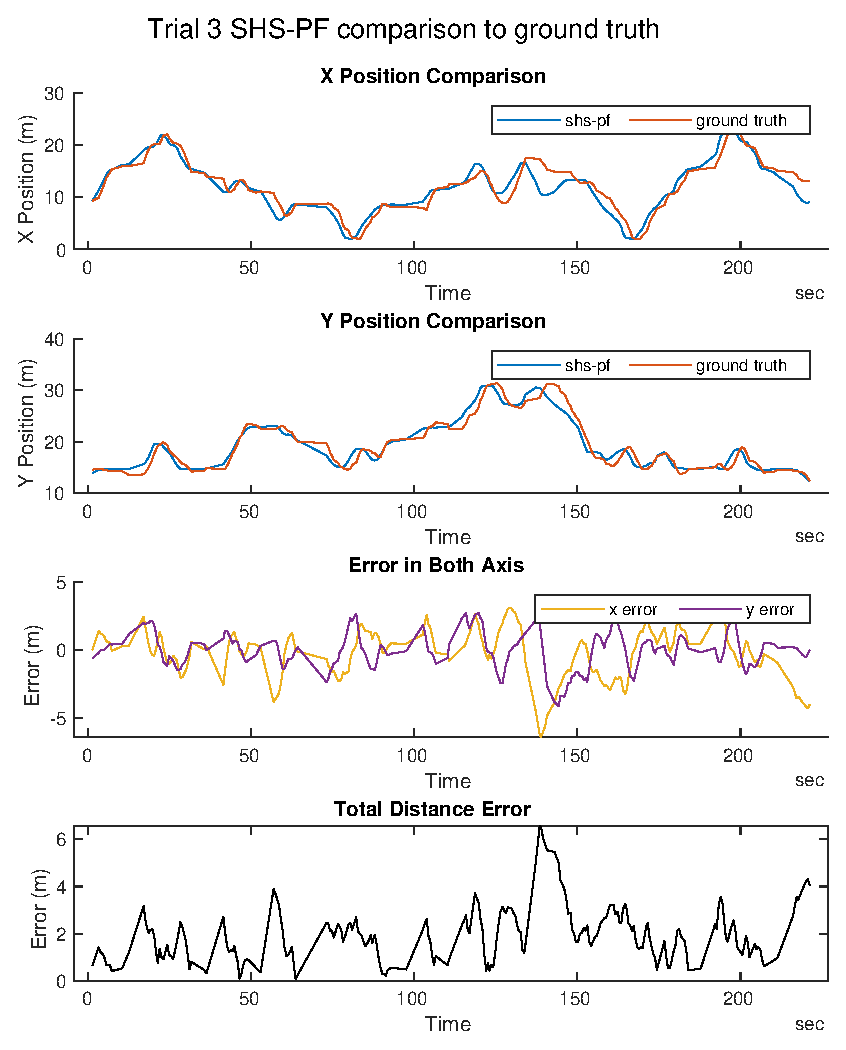
\includegraphics[width=\linewidth]{images/20201029_1804_shs-pf_trial_3_1}
		\caption{axis comparison}
		\label{fig:shspf_trial3_comparison}
	\end{subfigure}
	\caption{SHS-PF comparison of trial 3 with ground truth \textcolor{red}{change legends}}
	\label{fig:shspf_trial3_shs_gt_comparison}
\end{figure}
\begin{figure}[H]
	\centering
	\begin{subfigure}[t]{.45\textwidth}
		\centering
		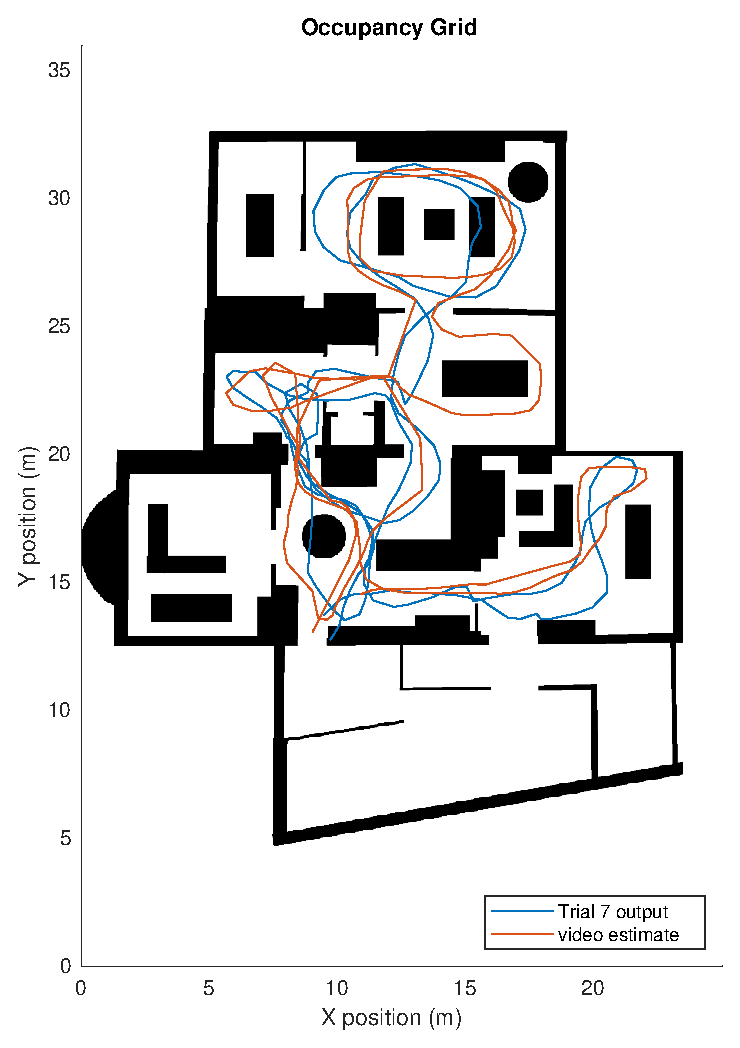
\includegraphics[width=0.9\linewidth]{images/20201118_1908_trial7_output_2}
		\caption{trajectory comparison}
		\label{fig:shspf_trial7_on_map}
	\end{subfigure}
	\begin{subfigure}[t]{.45\textwidth}
		\centering
		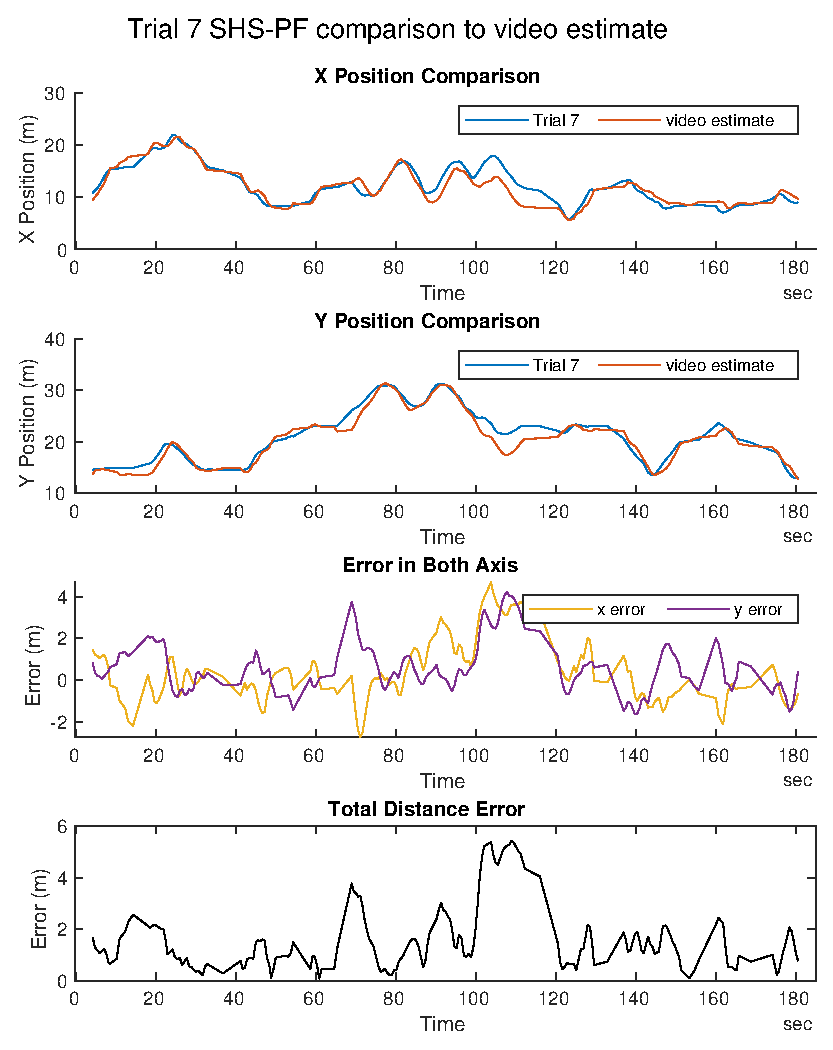
\includegraphics[width=\linewidth]{images/20201118_1908_trial7_output_1}
		\caption{axis comparison}
		\label{fig:shspf_trial7_comparison}
	\end{subfigure}
	\caption{SHS-PF comparison of trial 2 with ground truth}
	\label{fig:shspf_trial7_shs_gt_comparison}
\end{figure}
\newpage
\begin{figure}[H]
	\centering
	\begin{minipage}{.45\textwidth}
		\centering
		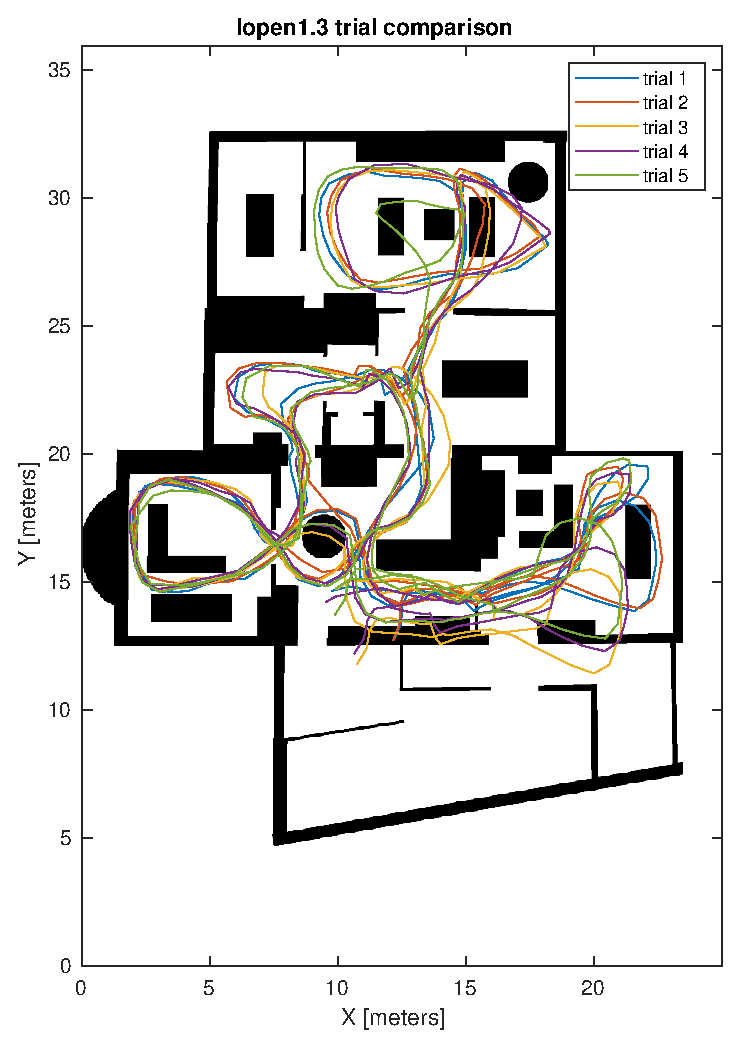
\includegraphics[width=\linewidth]{images/20201107_1142_trial_comparison_3}
		\caption{}
		\label{fig:202011071142trialcomparison3}
	\end{minipage}%
	\begin{minipage}{.45\textwidth}
		\centering
		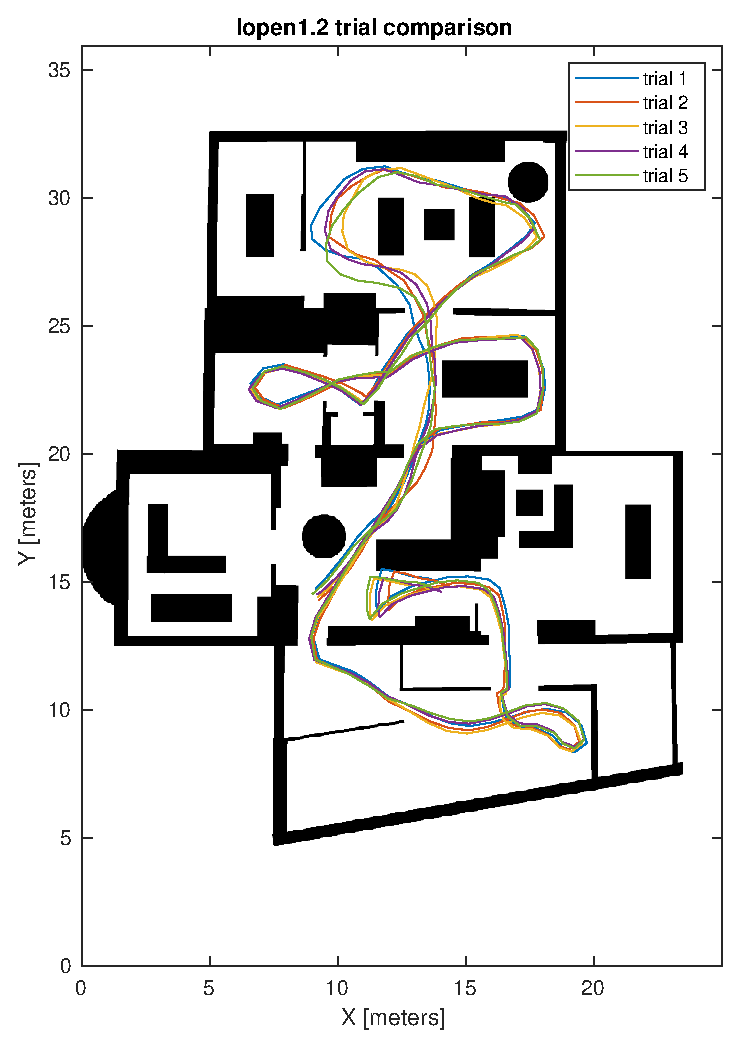
\includegraphics[width=\linewidth]{images/20201107_1142_trial_comparison_2}
		\caption{}
		\label{fig:202011071142trialcomparison2}
	\end{minipage}
\end{figure}


\begin{figure}[H]
	\centering
	\begin{minipage}{.45\textwidth}
		\centering
		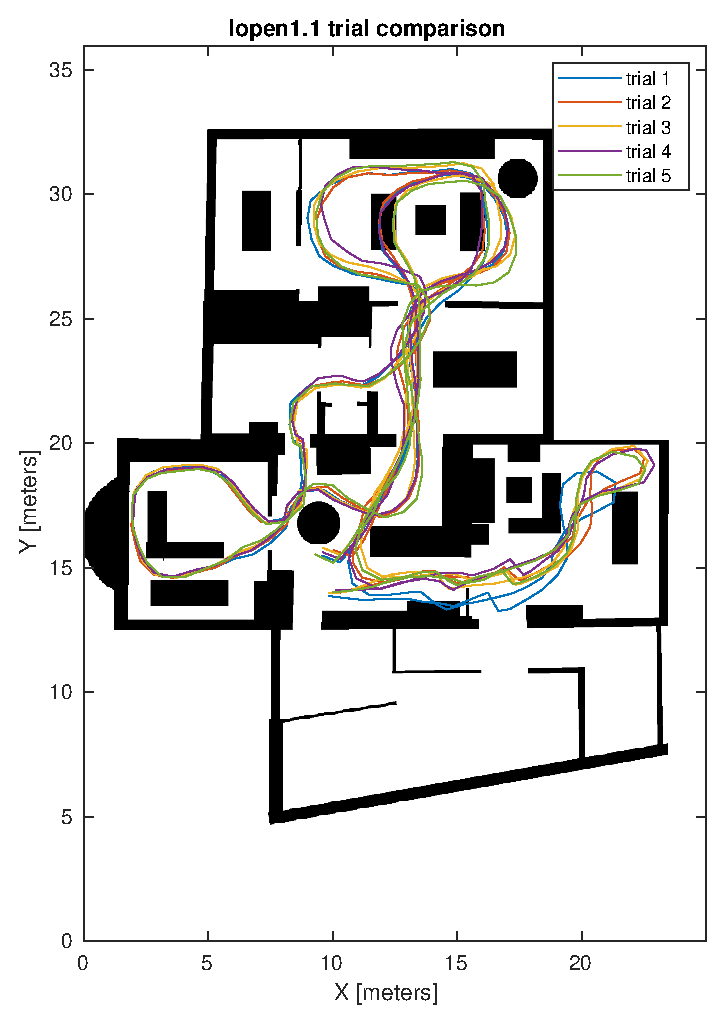
\includegraphics[width=\linewidth]{images/20201107_1142_trial_comparison_1}
		\caption{}
		\label{fig:202011071142trialcomparison1}
	\end{minipage}
\end{figure}

\section{Answering Research Questions}

\textcolor{cyan}{this will depend on the the eventual research questions that are found}

\section{Future Work}

{\color{purple}
\textbf{Step detection}
\begin{itemize}
	\item using data from \cite{Salvi2018} determine if parameters found are also the best parameters for the implementation used in this thesis.
	\item Step detection is a form of activity recognition, investigate if other machine learning techniques can perform better  
	\item testing was performed walking on a hard floor and it will be necessary to investigate softer surfaces like carpet or grass.
	\item Determine robustness against more complex movements
\end{itemize}

\textbf{Step length estimation}
\begin{itemize}
	\item generate more first hand data, maybe in a motion capture lab  
	\item use \cite{Bayev2019}, a data set that has recently been made to develop smartphone based pedestrian navigation 
	\item make the assumption that step length is constant and determine effect on performance
	\item when making a turn both feet do not travel the same distance. The inside foot will make a smaller step, while the outer a large one. Determine how turning affects the step length estimation.
\end{itemize}

\textbf{Orientation estimation}
\begin{itemize}
	\item use the method of \cite{Michel2018} to handle magnetic field disturbances
\end{itemize}

\textbf{Step heading estimation}
\begin{itemize}
	\item The testing was limited to one carrying mode, so that the yaw of the device would represent the direction in which the test subject is moving. Step heading estimation will need to be applied in order for the phone to be in other carrying modes.
\end{itemize}

\textbf{Particle filter}
\begin{itemize}
	\item Test without furniture or with a different probability density for furniture
	\item decrease probability close to walls since people do not generally walk close to walls
	\item different representation of map, instead of grid based more node and edge approach. 
	\item be able to detect when moving to a different floor
	\item combine other drift reduction methods
	\item initialize particles over whole map instead of defining a starting point.
	\item find a way to use less particles in order to be implementable on portable device. Above solutions could already help with this.
\end{itemize}

\textbf{Activity Recognition}
\begin{itemize}
	\item Detect more useful activities that can be used as additional particle filter measurement update. For example, climbing stairs for only smartphone sensors, or more intricate activities such as cooking
\end{itemize}

\textbf{Testing}
\begin{itemize}
	\item different building testing. The current contained may different ways of walking around, while other buildings with more corridor structures are more restrictive. Potentially the SHS-PF technique could have better performance in these settings.
	\item better ground truth determination for both positioning and orientation. ORB-SLAM2 was tried but could not get it to work with footage from phone.
	\item online calculation of position on device
	\item test with different people to determine how user sensitive this is.
\end{itemize}}
